\section{Results}
\label{sec:results}
The results on only a subset of our benchmarks are presented here for
lack of space.  
\begin{figure}[h!b]
\centering
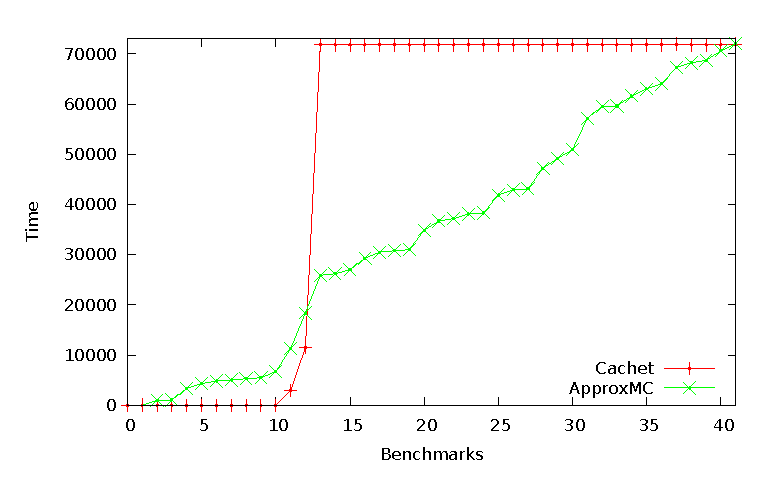
\includegraphics[scale=0.7]{time.eps}
\caption{Performance comparison between {\ApproxMC} and {\Cachet}. The
  benchmarks are arranged in increasing order of running time of
  {\ApproxMC}.}
\label{fig:perfomance_comparisons}
\end{figure}
Figure~\ref{fig:perfomance_comparisons} shows how the running times of
{\ApproxMC} and {\Cachet} compared on this subset of our benchmarks.  The
y-axis in the figure represents time in seconds, while the x-axis
represents benchmarks arranged in ascending order of running time of
{\ApproxMC}.  The comparison shows that although {\Cachet} performed
better than {\ApproxMC} initially, it timed out as the ``difficulty"
of problems increased.  {\ApproxMC}, however, continued to return
bounds with the specified tolerance and confidence, for many more
difficult and larger problems.  Eventually, however, even {\ApproxMC}
timed out for very large problem instances.  Our experiments clearly
demonstrate that there is a large class of practical problems that lie
beyond the reach of exact counters, but for which we can still obtain
counts with $(\varepsilon, \delta)$-style guarantees in reasonable
time.  This suggests that given a model counting problem, it is
advisable to run {\Cachet} initially with a small timeout.  If
{\Cachet} times out, {\ApproxMC} should be run with a larger timeout.
Finally, if {\ApproxMC} also times out, counters with much weaker
guarantees but shorter running times, such as bounding counters,
should be used.

\begin{figure}[h!b]\centering
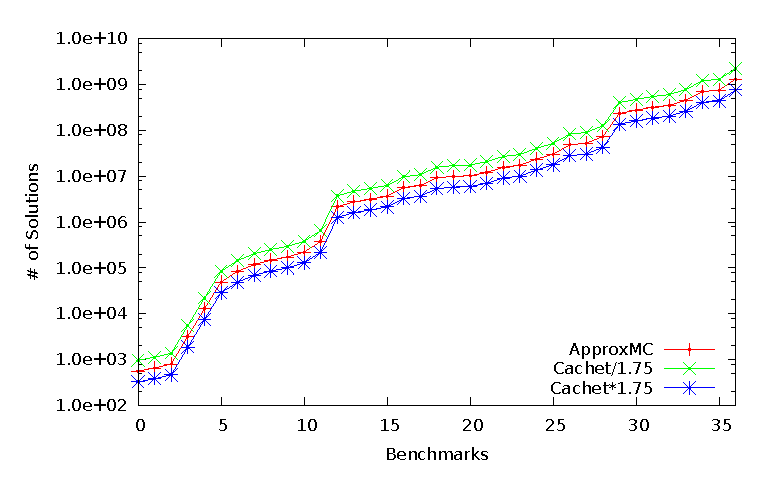
\includegraphics[scale=0.7]{quality.eps}
\caption{Quality of counts computed by {\approxMC}. The benchmarks are
  arranged in increasing order of model counts.}
\label{fig:quality_comparison}
\end{figure}
\begin{figure}[h!b]
\centering
\includegraphics[scale=0.7]{bounding.eps}
\caption{Comparison of interval sizes from {\approxMC} and those from
  bounding counters. The benchmarks are arranged in increasing order
  of model counts.}
\label{fig:bounding_comparisons}
\end{figure}
Figure \ref{fig:quality_comparison} compares the model count computed
by {\ApproxMC} with the bounds obtained by scaling the exact count
obtained from {\Cachet} by the tolerance factor ($1.75$) on
a subset of our benchmarks. The y-axis in this figure represents the
model count on a log-scale, while the x-axis represents the
benchmarks arranged in ascending order of the model count.
%
%
%
%
The figure shows that in all cases, the count reported by {\ApproxMC}
lies within the specified tolerance of the exact count.  Although we
have presented results for only a subset of our benchmarks ($37$
in total) in Figure~\ref{fig:quality_comparison} for reasons of
clarity, the counts reported by {\ApproxMC} were found to be within
the specified tolerance of the exact counts for \emph{all} $95$
benchmarks for which {\Cachet} reported exact counts.  %
%
%
We also found that the $L_1$ norm of the relative
error, considering all $95$ benchmarks for which {\Cachet} returned
exact counts, was $0.033$.  Thus, {\ApproxMC} has approximately $4\%$
error in practice -- much smaller than the theoretical guarantee of
$75\%$ with $\varepsilon = 0.75$.
  
Figure~\ref{fig:bounding_comparisons} compares the sizes of intervals
computed using {\ApproxMC} and using state-of-the-art bounding
counters (as described in Section~\ref{sec:experiment}) on a subset of
our benchmarks.  The comparison clearly shows that the sizes of
intervals computed using {\ApproxMC} are consistently smaller than the
sizes of the corresponding intervals obtained from existing bounding
counters.  Since smaller intervals with comparable confidence
represent better approximations, we conclude that {\approxMC} computes
better approximations than a combination of existing bounding
counters. In all cases, {\approxMC} improved the upper bounds from {\MiniCount} significantly; it also improved lower bounds from {\SampleCount} and {\MBound} to a lesser extent. For details, please refer to the full version. 
%

%
%
%
%
%
%
%
%
%
%
%
%
%
%
%
%
%
%
%
%
%
%
%
%
%
%
%
%
%
%
%
%
%
%
%
%
%
%
%
%
%
%
%
%
%
%
%
%
%
%
%
%
%
%
%
%
%
%
%
%
%
%
%
%
%
%
%
%
%
%
%
%
%
%
%
%
%
%
%
%
%
%
%
%
%
%
%
%
%
%
%
%
%
%
%
%
%
%
%
%
%
%
%
%
%
%
%
%
%
%
%
%
%
%
%
%
%
%
%
%
